% 博客园,繁星间漫步,陆巍的博客
\documentclass{ctexart}

\usepackage{graphics}% 图形支持
\usepackage{tikz}
\usetikzlibrary{shapes.geometric, positioning}


% ------------------ 开始 -------------------

\begin{document}
  \begin{tikzpicture}
    \node[
      circle,
      minimum size = 100mm,
      path picture = {
        \node at (path picture bounding box.center)
        {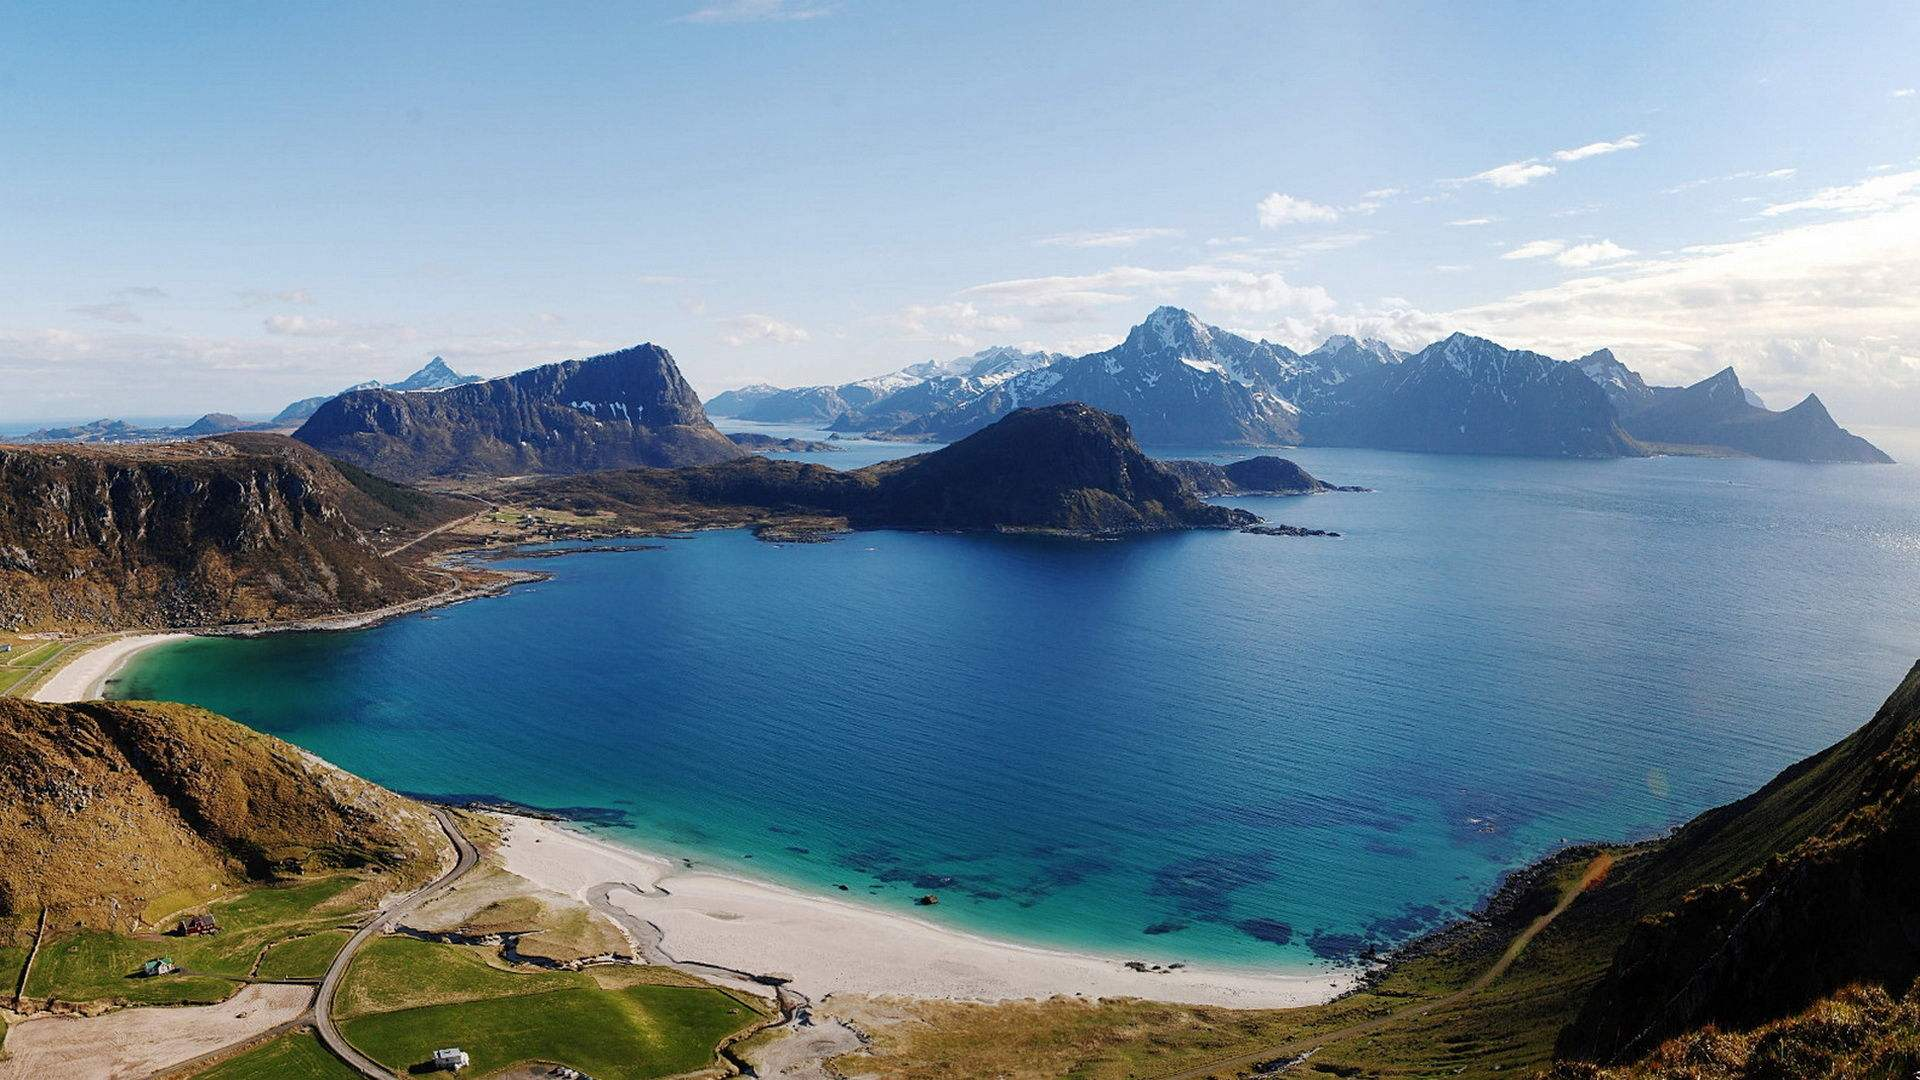
\includegraphics[width = 280mm]{images/cover2.png}};
      }
    ] {};
  \end{tikzpicture}
  
  \begin{tikzpicture}
    \node[
      isosceles triangle,
      isosceles triangle stretches,
      minimum size = 90mm,
      path picture = {
        \node at (path picture bounding box.center)
        {
\includegraphics[height = 100mm]{images/cover1.png}};
      }
    ] {};
  \end{tikzpicture}

\end{document}
